\section{OSI MODELİ (OSI KATMANLARI)}
Bir bilgisayardan gönderilen bir bilginin diğer bilgisayara nasıl ulaştığını anlatmak için tasarlanmıştır.
İletişimi 7 katmanlı mimarı ile tanımlar.
Ağ elemanlarının nasıl çalıştığını ve verinin iletimi sırasında hangi işlemlerden gectiğini kavramak için kullanılan rehberdir.
OSI Katmanlarının mantığını anlamak ağları planlamak, ağ üzerinden çalışan program yazmak ve ağ sorunlarını çözmek için önemlidir.

\subsection{Katmanlar}
\begin{enumerate}
	\item \hyperref[subsubsec:fiziksel_katmanlar]{ Fiziksel (Physical)}
	\item \hyperref[subsubsec:veri_bagi_katmani]{Veri Bağı (Data link)}
	\item \hyperref[subsubsec:ag_katmani]{Ağ (IP)}
	\item \hyperref[subsubsec:tasima_katmani]{Taşıma (Transport)}
	\item Oturum (Session)
	\item Sunum (Presentation)
	\item \hyperref[subsubsec:tasima_katmani]{Uygulama (Application)}
\end{enumerate}

\subsubsection{Fiziksel Katmanlar}\label{subsubsec:fiziksel_katmanlar}
Haberleşme kanalının elektriksel ve mekanik olarak tanımlandığı katmandır.
Bir uçtan gönderilen sinyalin karşı uca iletilmesinden sorumludur.
Sayısal haberleşmede en küçük birim bit olduğundan bu katmanın hızı \textbf{(bps) (b/s) bit/saniye} cinsindendir.
Birinci katman donanımları:
\begin{enumerate}
	\item Bakır ve fiber optik kablolar
	\item RF (Antenler)
	\item Sinyali(işareti) elektrik olarak yükselten ve çoklayan HUB cihazları
	\item Kablosuz iletişimde kullanılan hava
\end{enumerate}

\subsubsection{Veri Bağı Katmanı}\label{subsubsec:veri_bagi_katmani}
Verinin fiziksel ortamdan güvenli bir şekilde taşınmasından sorumlu olan katmandır.
Kaynaktan çıkan verilerin(bitler) hedefe ulaşan verilerle aynı olup olmadığını sınayan sistemler kullanılır.
En çok kullanılan hata bulma algoritmaları \textbf{eşlik biti (parity check)} ve \textbf{CRC algoritmasıdır}.
Verinin doğru olup olmadığına bakmaz, sadece sağlamlığını kontrol eder.
Bu katmanda üst katmandan gelen veriler çerçeve (frame) adı verilen paketleme işlemini tabi tutulur.
Kapsülleme de denir.
Birbirine doğrudan bağlı ağ cihazlarının aynı kapsülleme yöntemini (ikinci katman protokolünü) kullanması gerekir.

\begin{table}[h]
	\centering
	\begin{tabular}{|c|c|c|}
		\hline
		Kaynak & Veri & Hata Denetimi \\
		\hline
	\end{tabular}
	\caption{Kapsülleme}
	\label{tab:table_kapsulleme}
\end{table}

\subsubsection*{Günümüzde en yaygın ikinci katman protokolleri}
\textbf{Yerel ağda (LAN)} : Ethernet \\
\textbf{Uzak ağlarda (WAN)} : AIM, PPP, Frame, Relay, Metroethernet
\subsection*{Anahtarlama}
\begin{enumerate}
	\item[$\blacksquare$] \textbf{Devre Anahtarlama}: Veri aktarımı, fiziksel değişiklikle yapılır.
	\item[$\blacksquare$] \textbf{Paket Anahtarlama}: Veri aktarımı, her bir veri paketi için hesaplanarak, yazılımsal olarak yapılır.
\end{enumerate}
Ethernet protokolünde kaynak ve hedef adresleri olarak MAC adresi (fiziksel adresi) kullanılır. Çakışmaları engellemek için aynı ağda iki MAC adresi olmamalıdır.

Anahtarlar (switch) bu katmanda çalışır.
Anahtarlar portlarına bağlı olan cihazların MAC adreslerini bilmek zorundadır (otomatik öğrenir).
Bu şekilde iki farklı portu arasındaki trafiği diğer cihazlar görmeden aktarabilirler. \textbf{HUB'lardan en önemli farkı budur}.

\subsubsection{AĞ Katmanı (IP)}\label{subsubsec:ag_katmani}
İnternet dünyanın farklı yerlerindeki ağlar üzerinden erişebilir kiler katman budur.
Kaynak ve hedef olarak IP\footnote{IP => Internet Protocol} adresi kullanılır.
IP yönlendirilebilir bir protokol olduğundan her türlü veri aağı üzerinden haberleşmeye olarak sağlanır.
Bu katman en önemli görevi yönlendirme işlemidir.
Yönlendirme işlemi birden fazla ağ arayüzüne (network interface) sahip olan yönlendirici(router) adı verilen cihazlar tarafından yapılır.
IP internetin temel protokolüdür.
Yani bir PC internete bağlanacaksa IP'yi mutlaka biliyor olmalıdır.
Bazı anahtarlar üçüncü katmanda da çalışabilmektedir.
\begin{figure}[ht]
	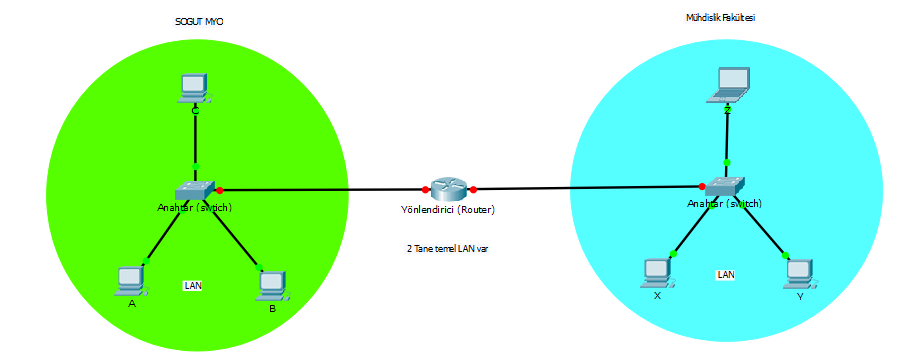
\includegraphics[width=15cm]{images/ip_katman}
	\caption{AĞ Katmanı}
	\label{fig:exemple_for_network_model}
\end{figure}
\begin{enumerate}
	\item[$\blacksquare$] \textbf{A,B,C} aynı ağdadır. Birbirleriyle MAC adresleriyle haberleşir (2. katman).
	\item[$\blacksquare$] \textbf{X,Y,Z} aynı ağdadır. Birbirleriyle MAC adresleriyle haberleşir (2. katman).
\end{enumerate}
\begin{figure}[ht]
	\centering
	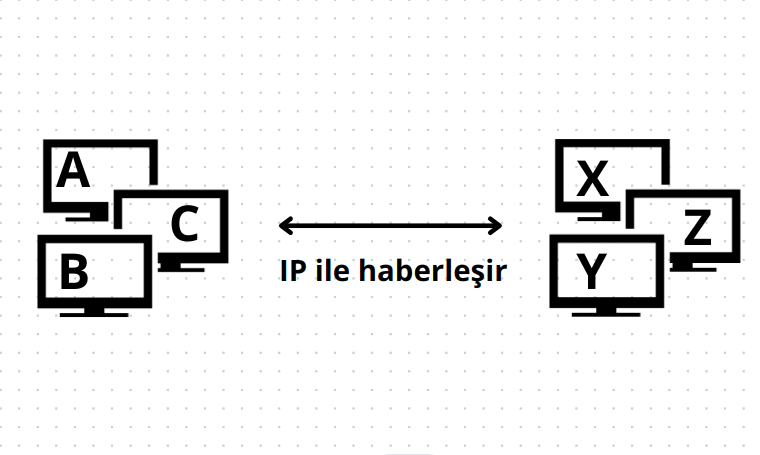
\includegraphics[width=10cm]{images/ip_communication}
	\label{fig:exemple_for_ip_communication}
\end{figure}
\begin{enumerate}
	\item[!] \textbf{En küçük birimine paketleme denir.}
\end{enumerate}

\subsubsection{Taşıma Katmanı}\label{subsubsec:tasima_katmani}
İnternette IP üzerinde kullanılan 2 tane 4. katman protokolü vardır.
Bunlar \textcolor{red}{\textbf{TCP}} ve \textcolor{red}{\textbf{UDP}} dir.
Bu katman uygulama programları için seri iletişim kanalları kuran katmandır.
Bu kanallar port adı verilen servis numaralarıyla kurulur.

\textbf{TCP}\footnote{TCP => Transmission Control Protocol}: Bağlantı temelli bir protokoldür. Trafik başlamadan önce karşıdaki uca müsait olup olmadığı sorulur.
Bu yönüyle telefon görüşmesine benzer.

\textbf{UDP}\footnote{UDP => User Datagram Protocol}: Bağlantı temelli değildir. Trafik doğrudan başlatıldığı için paketlerin iletimi garanti edilmez.
SMS gönderimine benzetilebilir. Özellikle gerçek zamanlı görüntü ve ses taşıma uygulamalarında elverişlidir.
\textbf{TCP}'ye göre daha \textbf{hızlıdır}.

\textbf{Örnek}: 3 way handshaking - 3 aşamalı el sıkışma
\begin{figure}[ht]
	\centering
	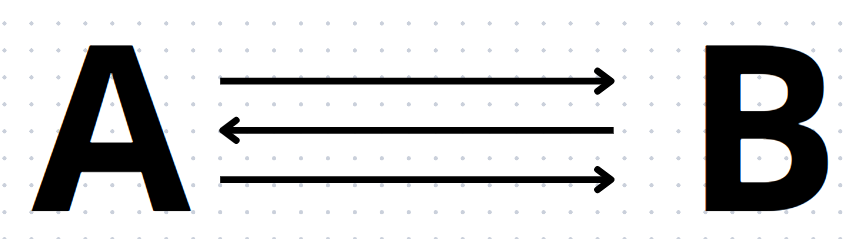
\includegraphics[width=10cm]{images/tcp_example}
	\caption{TCP Protokolü}
	\label{fig:tcp_example}
\end{figure}
Oturum açıldıktan sonra ilk olacak
- Veri kaç parçada gönderilecek \\
1GB filmi \\
80 segmentte $\Rightarrow$ (1180 2180 .... 80/80) bunlar paketlenir.

\textbf{TCP}'de sadece yavaşlama olacak görürüz.
En önemli avantajı budur.

\begin{figure}[ht]
	\centering
	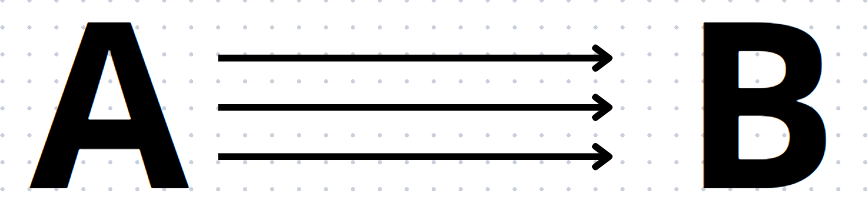
\includegraphics[width=10cm]{images/upd_example}
	\caption{UDP Protokolü}
	\label{fig:upd_example}
\end{figure}
\textbf{UDP}'nin avantajı hızlı  \textbf{TCP}'ye göre. Dezavantajı ise güvensiz.

\textbf{Örneğin}: İnternetten radyo dinleyeceğiz bunu \textbf{UDP} ile dinlemek zorundayız, çünkü GB belli değil.
\textbf{TCP}'de önemlidir.

\tab Dördüncü katmanın bir başka görevi de üst katmanlardan gelen veriyi bölümleyerek daha küçük parçalara ayırmaktır.
Bu parçalara \textbf{segment} denir.

\begin{table}[ht]
	\centering
	\begin{tabular}{|c|c|c|}
		\hline
		TCP                      & UDP        \\
		\hline
		Güvenli ( oturum temelli ) & Oturum yok \\
		\hline
		Yavaş                      & Hızlı      \\
		\hline
	\end{tabular}
	\caption{TCP vs UDP}
	\label{tab:tcp_vs_upd}
\end{table}

\subsubsection{Uygulama Seviyesi Katmanlar}\label{subsubsec:application_model}
Aslında uygulama seviyesi sadece 7. katmandır.
Ancak 5 ve 6 yaygın kullanılmadığından ve farklı uygulamalar arasında standart olmadığından bu derste üçüncu tek başlkta inceliyoruz.
\begin{figure}[!ht]
	\centering
	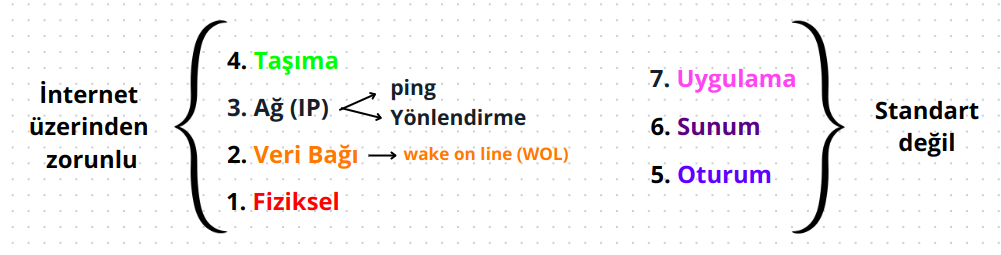
\includegraphics[width=17cm]{images/osi_example}
\end{figure}
Uygulama programları genellikle 7. katmanda ulaşmakta ve genellikle doğruden 4. katman ile iletişime geçmektedir.

\textbf{\textcolor{blue}{TELNET}}: Ağlarda yönetim ve kontrol amaclı kullanılır.
Ağ cihazlarının genellikle tamamı \textbf{telnet} ile yönetimi destekler.
2 cihaz arasında 4. katmanda bağlantı (erişebilirlik) kontrolü yapmak için \textbf{telnet} kullanılır.

** \textbf{Port tarama uygulamaları}\\
4. katmanda açık olan \textbf{\textcolor{red}{TCP/UDP}} portlarını tarar.

\textbf{\textcolor{blue}{nmap}}: \textbf{TCP} yada \textbf{UDP}'ye kadar \textbf{0-65536}'ye kadar port taraması yapar.


\begin{table}[ht]
	\centering
	\begin{tabular}{lll}

		\textbf{OBS}       & \textbf{Uzak masaüstu}  & \textbf{nmap -> OS dedikten } \\
		\hline
		Port tarama          & TCP 3389                & obs.bilecik.edu.tr            \\
		79.123.244.212 -> IP & 79.123.244.212 start IP & cevaplar                      \\
		TCP 80 open          & 79.123.244.212 end IP   & tahmin                        \\

	\end{tabular}
	\caption{Örnek}\label{tab:table}
\end{table}

\subsubsection{Aktarım Verimliliği}
\begin{figure}[!ht]
	\centering
	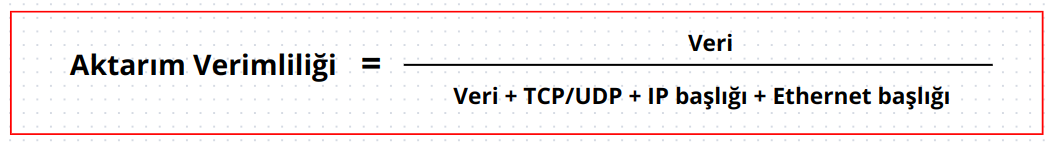
\includegraphics[width=17cm]{images/transmission_example}
\end{figure}

\begin{enumerate}
	\item[!] Veri bloğu ne kadar büyürse, verim o kadar artar.
\end{enumerate}

\textbf{\textcolor{red}{MTU\footnote{MTU => Maximum Transmission Unit}}}: Maksimum veri miktarını belirler. 
Ethernet bağlarında MTU değeri varsayılan olarak \textbf{1500 byts/kapsül}

\textbf{\textcolor{red}{PPL\footnote{PPL => Time to Live (Yaşam süresi)}}}: Paketlerin Ağda sonsuz kadar dolaşmaması için geçen süredir.\\
PPL değeri genellikle \textbf{128}'dir.

! Paket noktalar arasında her aktarıldığnda \textbf{PPL değeri azalır}.
